\documentclass[8pt,a4paper]{article}

\usepackage[a4paper, margin=1in]{geometry}

\usepackage[utf8]{inputenc}
\usepackage{amsmath, mathtools}
\usepackage{amsfonts}
\usepackage{amssymb}
\usepackage{nicefrac}
\usepackage{graphicx}
\usepackage{float}
\usepackage{pdfpages}
\usepackage{leftindex}
%\usepackage{showlabels} % show the reference labels
%\usepackage{hyperref} % show reference links
\usepackage[hidelinks]{hyperref} % hide reference links
\usepackage[makeroom]{cancel}

\begin{document}

	\title{Fourier Transform Spectroscopy with a Michelson Interferometer}
	\author{James Bounds}
	\maketitle
	
	This document provides the theoretical background of the Fourier Transform Spectroscopy (FTS) algorithms implemented in this package. The software is designed to convert raw interferogram time-series data into optical power spectra by accounting for non-linear stage velocities via interpolation.
	
	\section{Michelson Interferometer Physics} \label{sec:wl_wavelength}
	
	The core of the signal processing relies on the interference pattern produced by a Michelson interferometer. In a standard configuration, an incoming electric field $E_{\mathrm{in}}$ is split into two paths: a fixed arm (length $D$) and a movable arm (length $D + x$). This basic configuration is shown in Fig. \ref{fig:wl_michelsonsimple}. Incoming light is split into two paths using a beam splitter. These two paths traverse twice the two arms of the interferometer, and are recombined using the same beam splitter onto a photodetector.
	\begin{figure}[H]
		\centering
		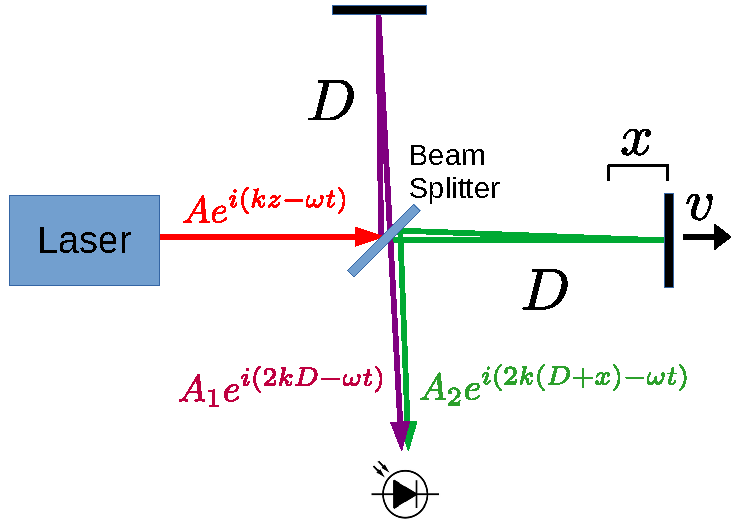
\includegraphics[width=0.5\linewidth]{diagrams/wl_michelsonSimple}
		\caption{A simplified configuration of a scanning Michelson interferometer with monochromatic input. A beam is split into two paths (shown in green and purple) by a beam splitter. The path shown in purple traverses a distance of $2D$, while the green beam travels a length $2(D+x)$ before being recombined at the beam splitter. Due to the time varying delay between the beams, a sinusoidal pattern in time is observed on the photodetector.}
		\label{fig:wl_michelsonsimple}
	\end{figure}
	
	\subsection{Monochromatic Signal}
	
	The incoming electric field can be described using the phasor
	\begin{equation}
		E_\mathrm{in} = A e^{i(kz - \omega t)}
	\end{equation}
	where the above quantities are
	\begin{itemize}
		\item $k$ -- The wave vector, $k=2\pi/\lambda$
		\item $A$ -- The beam electic field amplitude, related to the time averaged intensity by $I = \frac{c\epsilon_0 n}{2} \, \vec{\mathbf{E}} \cdot \vec{\mathbf{E}}^*$
		\item $z$ -- The propagation distance along the beam (we are ignoring transverse profile here)
		\item $\omega$ -- The angular optical frequency of the light, $\omega = 2\pi f$
		\item $t$ -- the time dependence
	\end{itemize}
	
	After traversing the fixed arm for a total distance of $2D$, the contribution of light at the output of the beam splitter from this path is
	\begin{equation}
		E_1 = A_1 e^{i(2kD - \omega t)}
	\end{equation}
	while the other path gives the contribution
	\begin{equation}
		E_2 = A_2 e^{i(2k(D+x) - \omega t)} = A_2 e^{2ikx}e^{i(2kD - \omega t)}
	\end{equation}
	The photodetector is exposed to the sum of the two fields
	\begin{align}
		E_p = E_1 + E_2 &= A_1 e^{i(2kD - \omega t)} + A_2 e^{2ikd}e^{i(2kD - \omega t)} \nonumber\\
		&= \left(A_1 + A_2 e^{2ikx}\right)e^{i(2kD - \omega t)}
	\end{align}
	
	It is clear that the field at the detector depends directly on the optical path difference (OPD) by the relation to the translation stage movement $\delta = 2x$ which is particular to the mechanical configuration of the delay. Proceeding forward, we use the OPD $\delta$ as it is independent of the particular mechanical configuration of the interferometer used to create the delay. The photodetector does not respond to the rapidly oscillating electric field, but to the time-averaged intensity, so the signal from the photodetector is proportional to
	\begin{align}
		I_p(\delta) = E_p^*E_p &= \left(A_1 + A_2 e^{ik\delta}\right)\left(A_1^* + A_2^* e^{-ik\delta}\right) \nonumber\\
		&= \left|A_1\right|^2 + \left|A_2\right|^2 + A_1A_2^*e^{-ik\delta} + A_1^*A_2e^{ik\delta}
	\end{align}
	The coefficients $A_{1,2}$ are in general complex and when written in the polar form $A_{1,2} = \left|A_{1,2}\right| e^{i\phi_{1,2}}$ the $\phi_{1,2}$ represent a constant phase shift of the output fields relative to the input field. Dropping the absolute value and writing the phase shift explicitly, the light intensity at the detector becomes
	\begin{equation}\label{wl_sig_monochromatic}
		\boxed{I_p(\delta) = A_1^2 + A_2^2 + A_1A_2\cos(k\delta + \phi_2 - \phi_1)}
	\end{equation}
	The intensity detected by the photodetector is an offset sinusoidal function of the OPD $\delta$. The amplitude of this sinusoid is maximized when the beams emerging from each arm have the same field strength (or equivalently the same intensity) which occurs when $A_1 = A_2$.
	
	For a broadband source, the total detected intensity $I(t)$ is the integral of all monochromatic components across the frequency spectrum:
	$$I(t) = I_0 + \int_{0}^{\infty} |\mathcal{A}(\omega)|^2 \cos\left(\frac{2\omega v t}{c} + \phi_0\right) d\omega$$
	where $v$ is the scanning velocity and $|\mathcal{A}(\omega)|^2$ is the target optical power spectrum.
	
	

	\section{Fourier Transform Spectroscopy (FTS)} \label{sec:wl_FTIR}

	The interferogram recorded by the photodetector for a monochromatic source was described in Eq. (\ref{wl_sig_monochromatic}). This result can be generalized to a broadband light source by treating the input field as a continuous superposition of monochromatic components. Neglecting phase-coherent beating between these components, the total interferogram intensity $I(t)$ is obtained by integrating the individual spectral contributions over the frequency spectrum:
	\begin{align} \label{wl_interferogram_incoherent}
		I(t) = \int_{0}^{\infty} |\mathcal{A}(\omega)|^2 \left[ 1 + \cos\big(k(\omega)\delta(t) + \phi_0(\omega)\big) \right] d\omega
	\end{align}
	The $\mathcal{A}(\omega)$ denotes the complex spectral amplitude of the input field $E_\mathrm{in}(t) = \mathcal{A}(\omega) e^{-i\omega t}$. Under the assumption of the dispersionless relation $k = \omega/c$ and a constant scanning velocity $v$, we have
	\begin{equation}
		\boxed{I(t) = I_0 + \int_{0}^{\infty} |\mathcal{A}(\omega)|^2 \cos\left(\frac{2\omega vt}{c} + \phi_0(\omega)\right) d\omega}
	\end{equation}
	Here $I_0$ represents the time-averaged power of the input light.
	
	The phase function $\phi_0(\omega)$ accounts for frequency-dependent phase delays introduced by optical elements, such as the beam splitter and mirrors. In FTS, the Michelson interferometer should be configured symmetrically to ensure that both arms impart identical phase delays, thereby minimizing any non-linear frequency dependence in $\phi_0(\omega)$. It is important to note that a linear term in $\phi_0(\omega)$ is physically equivalent to an additional optical path delay. Consequently, we proceed under the assumption that the interferometer is designed such that $\phi_0(\omega)$ is effectively constant, denoted as $\phi_0$.
	
	\section{Spectral Recovery via Fourier Transform}
	
	The software recovers the power spectrum by performing a Fourier Transform on the AC component of the interferogram. If the translation stage moves at a constant velocity, the frequency of the interferogram oscillations ($\omega_{\mathrm{int}}$) maps directly to the optical frequency:
	\begin{equation}
		\left|\mathcal{A}(\omega)\right|^2 = \mathcal{F}_t\left[I(t) - I_0\right](\omega)
	\end{equation}
	
	\subsection{Handling Non-Uniform Sampling (Velocity Correction)}
	In practical applications, mechanical instabilities in the translation stage cause the scanning velocity $v(t)$ to fluctuate. Applying a standard Fast Fourier Transform (FFT) directly to raw time-series data containing these fluctuations will result in spectral broadening and artifacts.
	
	\subsubsection{Implementation Strategy: Interpolation vs. NUFFT}
	While the Type-1 Non-Uniform Fast Fourier Transform (NUFFT) can extract spectra from irregularly sampled data, this package utilizes a \textbf{re-sampling approach} for computational efficiency:
	
	\begin{enumerate}
		\item \textbf{Reference Tracking:} A high-resolution reference laser interferogram is used to track the instantaneous OPD, $\delta(t)$, with precision.
	 	\item \textbf{Cubic Spline Interpolation:} The intensity signal $I(t)$ is re-mapped from the time domain onto a strictly uniform grid in the $\delta$ (optical path difference) domain.
	 	\item \textbf{FFT Execution:} Once linearized, the signal is processed using standard FFT algorithms.
	\end{enumerate}
	
	This method ensures spectral integrity and maintains high resolution even when the translation stage experiences non-linear velocity profiles, provided the reference laser signal is sampled at a sufficient rate for effective interpolation.
	
	\section{Tracking the Stage with the Reference Laser}
	In any physical Michelson interferometer, the scanning velocity $v(t)$ is rarely perfectly constant due to motor cogging, friction, or vibration. If these fluctuations are not corrected, the resulting interferogram contains non-linear phase modulation, which manifests as "ghosting" or artificial broadening in the final Fourier-transformed spectrum.
	
	To mitigate this, a reference laser (typically a stabilized HeNe or-diode laser) is directed through the same interferometer path as the test source, as seen in Fig. \ref{fig:wlwavemeter}. Because the frequency of the reference laser ($\omega_{ref}$) is known and extremely stable, its interferogram acts as a high-precision displacement transducer.
	
	\begin{figure}[H]
		\centering
		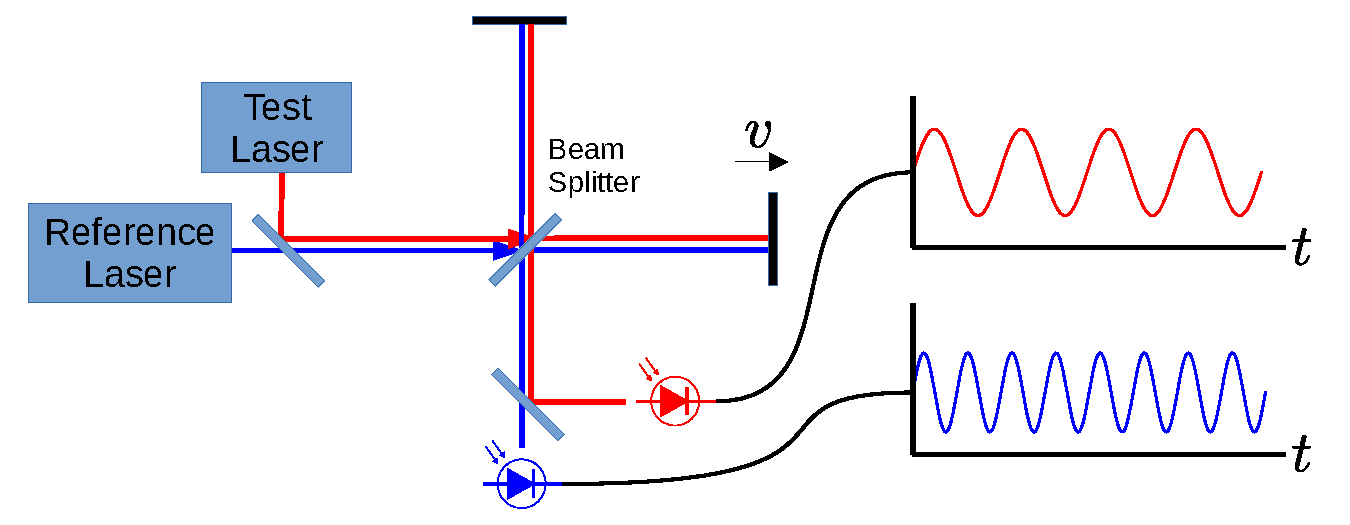
\includegraphics[width=0.75\linewidth]{diagrams/wl_wavemeter}
		\caption{Setup for the simultaneous capture of two interferograms using a Michelson interferometer. The reference laser allows for precise tracking of the translational stage, which can in general have a non-uniform velocity $v(t)$. The recording of these two signals allows for the high-precision measurement of wavelength ratios.}
		\label{fig:wlwavemeter}
	\end{figure}
	
	\subsection{The Tracking Algorithm}
	The software processes the reference and test signals using the following pipeline:
	
	\begin{enumerate}
		\item \textbf{Bandpass Filter:} The high-frequency oscillations of the reference laser interferogram are isolated using a digital bandpass filter centered near the oscillation frequency. This gives a clean reference signal centered on zero. 
		\item \textbf{Delay $\delta(t)$ Reconstruction}: By calculating the derivative of the reference phase identifying zero-crossings/peaks, the software reconstructs a continuous time-series of the actual Optical Path Difference, $\delta(t)$, rather than assuming a linear $x = vt$ relationship.
		\item \textbf{Temporal Mapping:} The primary test-laser signal is treated as being sampled at non-uniform intervals $\Delta \delta$. 
		\item \textbf{Interpolation (Linearization):} The primary test-laser signal is treated as being sampled at non-uniform intervals $\Delta \delta$. Using the reconstructed $\delta(t)$ map, the software applies a cubic spline interpolation. This re-samples the test-laser intensity from the distorted time-domain $I(t)$ onto a synthetic, uniform grid of $\delta$.
	\end{enumerate}
	
	\subsubsection{Result}
	By transforming the signal into the $\delta$-domain before applying the FFT, the software effectively "de-warps" the data. The resulting spectrum reflects the true optical power distribution $|\mathcal{A}(\omega)|^2$, mathematically canceling out the phase errors introduced by the translation stage's mechanical imperfections.
	
	\end{document}